\subsubsection{IS Auditor e IT Governance}

Esistono cinque indicatori per capire se l'azienda ha fatto un buon lavoro nel
veicolare i propri obiettivi ai lavoratori. È importante che i dipendenti
sappiano dare risposte
\begin{enumerate*}[label=\arabic*)]
\item a cosa è allineata la compagnia,
\item qual è la sua missione,
\item visione,
\item valori,
\item obiettivi e strategie.
\end{enumerate*}

Quando un dipendente non lo sa o
risponde ``solo per i soldi'' è un segnale negativo.

\paragraph*{IT} L'IT serve per potare avanti obiettivi strategici di business,
ed è importante sapere se l'IT è in grado di raggiungere le \textit{performance}
e gli obiettivi stabiliti. Inoltre sono presenti requisiti a cui essi devono
sottostare, come per esempio quelli legali o quelli legati alla qualità.

\paragraph*{Efficacia ed efficienza} L'efficienza è l'uso ottimale delle
risorse, l'efficacia è il raggiungimento degli obiettivi e dei requisiti
prefissati.


\subsubsection{Esercizi}

La parte di esercizi è disponibili in \ref{esSA:SO}

\part{Controlli di Sicurezza e Sicurezza del Software}

Questo modulo si concentra sui controlli di sicurezza del software. Per fare ciò
dovremo vedere il ciclo di vita del software, con un occhio alla sicurezza.
Partiremo dall'analisi dei requisiti, per andare all'analisi del rischio e per
finire con lo sviluppo del software.
Anche l'ambiente produttivo richiede attenzione: è importante il mantenimento da
parte di vista della sicurezza per non introdurre bug nel software.

\begin{figure}[h!]
        \begin{center}
                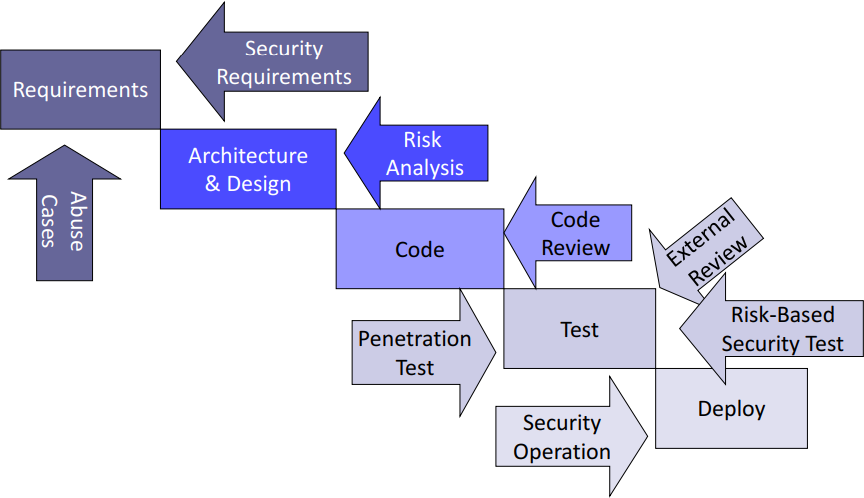
\includegraphics[width=\textwidth]{security_software_development}
        \end{center}
        \caption[La sicurezza nello sviluppo del software]{
         La sicurezza nello sviluppo del software. Nella figura
         \begin{enumerate*}[label=\alph*)]
		 \item ``Abuse cases'' (invece di use cases) si riferiscono ai
		 tipici casi in cui il sistema può essere flesso in chiara
		 violazione delle policy di sicurezza;
		 \item La Code review consiste anche nell'analisi statica;
		 \item Il Test sul software è inteso come penetration test, stress test, ecc.
		 \end{enumerate*}
		}
        \label{fig:security:software:development}
\end{figure}

Prima di procedere con lo studio dei vari controlli nei capitoli
\ref{cs:ac} e \ref{cs:aa}, analizzeremo nell'ambito del capitolo
\ref{Controlli} come si è evoluto il software e i conseguenti attacchi,
a partire da attacchi classici come il \textit{buffer overflow},
per arrivare a sfruttare errori nella codifica dei caratteri negli URL
degli indirizzi web.

\chapter{Controlli}
\label{Controlli}

\section{Controlli su input}

Ci sono diversi tipi di attacchi che sfruttano gli input, e questi sono:
\textbf{dati falsi}, \textbf{buffer overflow}\footnote{Si sfrutta l'allocazione
di memoria nei programmi per eseguire codice arbitrario. Molto difficile da
applicare ma molto efficace una volta riuscito l'attacco. Da spesso la
possibilità all'attaccante di ottenere il controllo della macchina. Vedere il
paper: \textit{Smashing The Stack For Fun And Profit.}}.

Per risolvere tutti questi problemi è necessario \textbf{validare l'input},
meglio se tramite le \textit{white list}, ovvero stendere una lista bianca in
cui tutto ciò che è scritto nella lista è accettato. Usare una \textit{black
list} è il complementare, e detta tutto ciò che non è possibile fare.
Ovviamente la seconda è meno restrittiva della prima.

\section{Interazioni insicure tra componenti}

Un attacco tipico è quando un attaccante riesce a ``intrufolarsi'' in una
comunicazione insicura, e riesce a trasmettere dati arbitrari.
Qual è la debolezza qui? È che la associazione tra dispositivi è stata eseguita
prima che per esempio uno dei due dispositivi vada in \textit{sleep}, e non
viene eseguita dopo. Quindi una possibile soluzione è eseguire il login, e poi
comunicare in maniera criptata.

L'hash garantisce integrity.

Un altro possibile attacco è quello dell'\textbf{SQL Injection}, dove un'intera
stringa SQL viene mandata tramite input, che non viene sanitizzato. Un attacco
simile con i comandi di sistema operativo si chiama \textbf{OS Command
Injection}. Tutti questi problemi vengono risolti separando i controlli dai
dati.

\section{Jail \& Sandbox}

\textbf{Jail:} il sistema operativo mette dei limiti sulle risorse che si
possono utilizzare.
Da qui viene ``Jailbreak''.\\
\newline
\textbf{Sandbox}: l'applicazione viene fatta girare in un ambiente controllato.


\section{Interazione insicura dei componenti}

Questo problema può essere visto anche quando la interazione dei componenti tra
loro è sicura, ma quando ne esistono molti potrebbero essere insicura.

Un attacco simile può essere il \textit{Cross-Site Scripting}, ovvero quando si
fa l'\textit{inject} di codice in una richiesta web.


Esistono attacchi anche su componenti che pensiamo sicure come l'SSL. Un
esempio è il \textit{SSL strip attack}.

Un \textbf{nonce} è un numero che non deve essere casuale, ma dev'essere unico.
Va bene che sia anche predicibile. Serve in tutti i livelli di
\textit{encryption} decenti.
